\subsection{Feature detection} \label{subsec:featuredetection}

Discriminative features allowing to recognize \ac{cap} from healthy tissue have to be first detected. This section will summarize the different strategies employed for this task. The feature type used is summarized in Tab. \ref{tab:feat} while Tab. \ref{tab:featrev} summed up which strategies were used by the different studies reviewed.

\begin{table*}
	\caption{Overview of the feature detection methods used in \ac{cad} systems.}
	\small
	\renewcommand{\arraystretch}{.9}
	\begin{tabular}{p{.7\linewidth} >{\centering\arraybackslash}p{.20\linewidth}}
		\hline \\ [-1.5ex]
		\textbf{Feature detection methods} & \textbf{Indexes} \\ \\ [-1.5ex]
		\hline \\ [-1.5ex]
		\textbf{\ac{mri} image:} & \\ \\ [-1.5ex]
		\quad \textit{Voxel-wise detection} &  \\ \\ [-1.5ex]
		\quad \quad Intensity-based & A \\
		\quad \quad Edge-based & \\
		\quad \quad \quad Prewitt operator & B$_1$ \\
		\quad \quad \quad Sobel operator & B$_2$ \\
		\quad \quad \quad Kirsch operator & B$_3$ \\
		\quad \quad \quad Gabor filtering & B$_4$ \\ 
		\quad \quad Texture-based & \\
		\quad \quad \quad Haralick features & C$_1$ \\
		\quad \quad \quad Fractal analysis & C$_2$ \\
		\quad \quad \quad \Ac{dct} & C$_3$ \\
		\quad \quad \quad Wavelet-based features & C$_4$ \\
		\quad \quad Position-based & D \\ \\ [-1.5ex]
		\quad \textit{Region-wise detection} &  \\ \\ [-1.5ex]
		\quad \quad Statistical-based & \\
		\quad \quad \quad Percentiles & E$_1$ \\
		\quad \quad \quad Statistical-moments & E$_2$ \\
		\quad \quad Histogram-based & \\
		\quad \quad \quad \Ac{pdf} & F$_1$ \\
		\quad \quad \quad \Ac{hog} & F$_2$ \\
		\quad \quad \quad Shape context & F$_3$ \\
		\quad \quad \quad \Ac{lbp} & F$_4$ \\
		\quad \quad Anatomical-based & G \\ \\ [-1.5ex]
		\textbf{\ac{dce} signal:} & \\ \\ [-1.5ex]
		\quad Whole spectra approach & H \\
		\quad Semi-quantitative approach & I \\
		\quad Quantitative approach &  \\
		\quad \quad Toft model & J$_1$ \\
		\quad \quad Brix model & J$_2$ \\
		\quad \quad Weibull function & J$_3$ \\
		\quad \quad Phenomenological universalities model & J$_4$ \\
		\\ [-1.5ex]
		\textbf{\ac{mrsi} signal:} & \\ \\ [-1.5ex]
		\quad Whole spectra approach & K \\
		\quad Quantification approach & L \\
		\quad Wavelet-based approach & M \\ \\ [-1.5ex]
		\hline
	\end{tabular}
	\label{tab:feat}
\end{table*}

\begin{table*}
\centering
\caption{Overview of the different features extracted by studies reviewed. The indexes of the features are presented in Tab. \ref{tab:feat}.}
\footnotesize
%\begin{adjustwidth}{-2.2cm}{}
\begin{threeparttable}
\renewcommand{\arraystretch}{1.5}
	%\rowcolors{3}{black!5}{white}	
	\begin{tabular}{c@{\hspace{2.5ex}}>{\columncolor[gray]{0.95}}c@{\hspace{2.5ex}}c@{\hspace{2.5ex}}>{\columncolor[gray]{0.95}}c@{\hspace{2.5ex}}c@{\hspace{2.5ex}}>{\columncolor[gray]{0.95}}c@{\hspace{2.5ex}}c@{\hspace{2.5ex}}>{\columncolor[gray]{0.95}}c@{\hspace{2.5ex}}c@{\hspace{2.5ex}}>{\columncolor[gray]{0.95}}c@{\hspace{2.5ex}}c@{\hspace{2.5ex}}>{\columncolor[gray]{0.95}}c@{\hspace{2.5ex}}c@{\hspace{2.5ex}}>{\columncolor[gray]{0.95}}c@{\hspace{2.5ex}}c@{\hspace{2.5ex}}>{\columncolor[gray]{0.95}}c@{\hspace{2.5ex}}c@{\hspace{2.5ex}}>{\columncolor[gray]{0.95}}c@{\hspace{2.5ex}}c@{\hspace{2.5ex}}>{\columncolor[gray]{0.95}}c@{\hspace{2.5ex}}c@{\hspace{2.5ex}}>{\columncolor[gray]{0.95}}c@{\hspace{2.5ex}}c@{\hspace{2.5ex}}>{\columncolor[gray]{0.95}}c@{\hspace{2.5ex}}c@{\hspace{2.5ex}}>{\columncolor[gray]{0.95}}c@{\hspace{2.5ex}}c@{\hspace{2.5ex}}>{\columncolor[gray]{0.95}}c@{\hspace{2.5ex}}}\hline
	%\hiderowcolors
%	\multirow{2}{*}{Index} & \multirow{2}{*}{Study} & \# & \multicolumn{4}{c|}{\ac{mri}-modality} & \multicolumn{2}{c|}{Strength of field} & \multicolumn{2}{c|}{Studied zones} & \multicolumn{3}{c|}{\ac{cad} stages} \\ \cline{4-14}
%	 & & patients & \ac{t2w} \ac{mri} & \ac{dce} \ac{mri} & \ac{dw} \ac{mri} & \ac{mrsi} & 1.5 T & 3.0 T & \ac{pz} & \ac{cg} & Img. Reg. & \ac{cade} & \ac{cadx}
	%\cline{2-25}
	%\multirow{2}{*}{Articles} & \multicolumn{16}{@{\hspace{2.5ex}}c|@{\hspace{2.5ex}}}{\ac{mri} images} & \multicolumn{6}{@{\hspace{2.5ex}}c@{\hspace{2.5ex}}|}{\ac{dce}} & \multicolumn{3}{@{\hspace{2.5ex}}c@{\hspace{2.5ex}}}{\ac{mrsi}} \\
	%\cline{2-26}	
	 Indexes & A & B$_1$ & B$_2$ & B$_3$ & B$_4$ & C$_1$ & C$_2$ & C$_3$ & C$_4$ & D & E$_1$ & E$_2$ & F$_1$ & F$_2$ & F$_3$ & F$_4$ & G & H & I & J$_1$ & J$_2$ & J$_3$ & J$_4$ & K & L & M \\ \hline \hline
	 %\showrowcolors %\tiny{$\triangle\bullet\diamond$}
		$[1]$ & \tiny{$\triangle--$} &  &  &  &  &  &  &  &  &  &  & \tiny{$\triangle--$} &  &  &  &  &  & \cmarksmall &  &  &  &  &  &  &  &  \\ \hdashline
		$[2]$ & \tiny{$\triangle--$} &  &  &  &  &  &  &  &  &  &  & \tiny{$\triangle--$} &  &  &  &  &  & \cmarksmall &  &  &  &  &  &  &  &  \\ \hdashline
		$[3]$ &  &  &  &  &  & \tiny{$\triangle--$} &  &  &  &  & \tiny{$--\diamond$} & \tiny{$--\diamond$} &  &  &  &  &  &  &  &  &  &  &  &  &  &  \\ \hdashline
		$[4]$ & \tiny{$\triangle-\diamond$} &  &  &  &  &  &  &  &  &  &  &  &  &  &  &  &  &  &  &  & \mmarksmall &  &  &  &  &  \\ \hdashline
		$[5]$ & \tiny{$\triangle-\diamond$} &  &  &  &  &  &  &  &  &  &  &  &  &  &  &  &  &  &  &  & \mmarksmall &  &  &  &  &  \\ \hdashline
		$[6]$ & \tiny{$\triangle-\diamond$} &  &  &  &  &  &  & \tiny{$\triangle-\diamond$} &  & \cmarksmall &  &  &  &  &  &  &  &  &  &  &  &  &  &  &  &  \\ \hdashline
		$[7]$ & \tiny{$--\diamond$} &  &  &  &  &  &  &  &  &  &  &  &  &  &  &  &  &  &  & \cmarksmall &  & \cmarksmall & \cmarksmall &  &  &  \\ \hdashline
		$[8]$ &  &  &  &  &  &  &  &  &  &  &  &  &  &  &  &  &  &  &  &  &  &  &  & \cmarksmall & \cmarksmall &  \\ \hdashline
		$[9]$ & \tiny{$\triangle-\diamond$} &  &  &  &  &  &  &  &  &  &  &  &  &  &  &  &  &  &  & \cmarksmall &  &  &  &  &  &  \\ \hdashline
		$[10]$ & \tiny{$\triangle-\diamond$} &  &  &  &  &  &  &  &  & \cmarksmall & \tiny{$\triangle\bullet\diamond$} & \tiny{$\triangle\bullet\diamond$} &  &  &  &  &  &  &  & \cmarksmall &  &  &  &  &  &  \\ \hdashline
		$[11]$ & \tiny{$\triangle-\diamond$} &  &  &  &  & \tiny{$\triangle\bullet\diamond$} &  &  &  & \cmarksmall & \tiny{$\triangle\bullet\diamond$} & \tiny{$\triangle\bullet\diamond$} &  &  &  &  & \cmarksmall &  &  & \cmarksmall &  &  &  &  &  &  \\ \hdashline
		$[12]$ & \tiny{$\triangle-\diamond$} &  &  &  &  &  &  &  &  &  &  &  &  &  &  &  &  &  &  &  & \cmarksmall &  &  &  &  &  \\ \hdashline
		$[13]$ &  &  &  &  &  &  &  &  &  &  &  &  & \tiny{$\triangle\bullet\diamond$} & \tiny{$\triangle\bullet\diamond$} & \tiny{$\triangle\bullet\diamond$} & \tiny{$\triangle\bullet\diamond$} &  &  &  & \mmarksmall &  &  &  &  &  &  \\ \hdashline
		$[14]$ &  &  &  &  &  &  & \tiny{$\triangle--$} &  &  &  &  &  &  &  &  &  &  &  &  &  &  &  &  &  &  &  \\ \hdashline
		$[15]$ &  &  &  &  &  &  & \tiny{$\triangle--$} &  &  &  &  &  &  &  &  &  &  &  &  &  &  &  &  &  &  &  \\ \hdashline
		$[16]$ &  &  &  &  &  &  &  &  &  &  &  &  &  &  &  &  & \cmarksmall &  &  &  &  &  &  & \cmarksmall &  &  \\ \hdashline
		$[17]$ &  &  &  &  &  &  &  &  &  &  &  &  &  &  &  &  &  &  & \cmarksmall & \cmarksmall &  & \cmarksmall & \cmarksmall &  &  &  \\ \hdashline
		$[18]$ & \tiny{$\triangle\bullet\diamond$} &  & \tiny{$\triangle\bullet\diamond$} & \tiny{$\triangle\bullet\diamond$} &  & \tiny{$\triangle\bullet\diamond$} &  &  &  &  & \tiny{$\triangle\bullet\diamond$} & \tiny{$\triangle\bullet\diamond$} &  &  &  &  &  &  & \cmarksmall & \cmarksmall &  &  &  &  &  &  \\ \hdashline
		$[19]$ & \tiny{$\triangle\bullet\diamond$} &  & \tiny{$\triangle\bullet\diamond$} & \tiny{$\triangle\bullet\diamond$} &  & \tiny{$\triangle\bullet\diamond$} &  &  &  &  & \tiny{$\triangle\bullet\diamond$} & \tiny{$\triangle\bullet\diamond$} &  &  &  &  &  &  & \cmarksmall & \cmarksmall &  &  &  &  &  &  \\ \hdashline
		$[20]$ & \tiny{$\triangle-\diamond$} &  &  &  &  &  &  &  &  &  &  &  &  &  &  &  &  &  &  &  & \mmarksmall &  &  &  &  &  \\ \hdashline
		$[21]$ & \tiny{$\triangle-\diamond$} &  &  &  &  &  &  &  &  &  &  &  &  &  &  &  &  &  &  &  & \mmarksmall &  &  &  &  &  \\ \hdashline
		$[22]$ &  &  &  &  &  &  &  &  &  &  &  &  &  &  &  &  &  &  &  &  &  &  &  & \cmarksmall & \cmarksmall &  \\ \hdashline
		$[23]$ &  &  &  &  &  &  &  &  &  &  & \tiny{$--\diamond$} & \tiny{$\triangle-\diamond$} &  &  &  &  &  &  &  & \mmarksmall &  &  &  &  &  &  \\ \hdashline
		$[24]$ &  &  &  &  &  &  &  &  &  &  &  &  &  &  &  &  &  &  & \mmarksmall &  &  &  &  &  &  &  \\ \hdashline
		$[25]$ &  &  &  &  &  &  &  &  &  &  &  &  &  &  &  &  &  &  & \cmarksmall &  & \cmarksmall &  &  &  &  &  \\ \hdashline
		$[26]$ &  &  &  &  &  &  &  &  &  &  &  &  &  &  &  &  &  &  &  &  &  &  &  & \cmarksmall &  &  \\ \hdashline
		$[27]$ &  &  &  &  &  &  &  &  &  &  &  &  &  &  &  &  &  &  &  &  &  &  &  & \cmarksmall &  &  \\ \hdashline
		$[28]$ &  &  &  &  &  &  &  &  &  &  &  &  &  &  &  &  &  &  &  &  &  &  &  & \cmarksmall &  &  \\ \hdashline
		$[29]$ &  & \tiny{$\triangle--$} & \tiny{$\triangle--$} & \tiny{$\triangle--$} &  & \tiny{$\triangle--$} &  &  &  &  &  & \tiny{$\triangle--$} &  &  &  &  &  &  &  &  &  &  &  & \cmarksmall &  &  \\ \hdashline
		$[30]$ &  & \tiny{$\triangle--$} & \tiny{$\triangle--$} & \tiny{$\triangle--$} &  & \tiny{$\triangle--$} &  &  &  &  &  & \tiny{$\triangle--$} &  &  &  &  &  &  &  &  &  &  &  & \cmarksmall &  &  \\ \hdashline
		$[31]$ &  &  &  &  & \tiny{$\triangle--$} &  &  &  &  &  &  &  &  &  &  &  &  &  &  &  &  &  &  &  &  & \cmarksmall \\ \hdashline
		$[32]$ &  & \tiny{$\triangle--$} & \tiny{$\triangle--$} & \tiny{$\triangle--$} &  & \tiny{$\triangle--$} &  &  &  &  &  & \tiny{$\triangle--$} &  &  &  &  &  &  &  &  &  &  &  & \cmarksmall &  &  \\ \hdashline
		$[33]$ &  & \tiny{$\triangle--$} & \tiny{$\triangle--$} & \tiny{$\triangle--$} & \tiny{$\triangle--$} & \tiny{$\triangle--$} &  &  &  &  &  & \tiny{$\triangle--$} &  &  &  &  &  &  &  &  &  &  &  & \cmarksmall &  &  \\ \hdashline
		$[34]$ &  &  &  &  &  &  &  &  &  &  &  &  &  &  &  &  &  & \cmarksmall &  &  &  &  &  &  &  &  \\ \hdashline
		$[35]$ &  &  & \tiny{$\triangle--$} & \tiny{$\triangle--$} &  & \tiny{$\triangle--$} &  &  &  &  &  & \tiny{$\triangle--$} &  &  &  &  &  & \cmarksmall &  &  &  &  &  &  &  &  \\ \hdashline
		$[36]$ &  &  & \tiny{$\triangle--$} & \tiny{$\triangle--$} &  & \tiny{$\triangle\bullet-$} &  &  &  &  &  & \tiny{$\triangle\bullet-$} &  &  &  &  &  & \cmarksmall &  &  &  &  &  &  &  &  \\ \hdashline
		$[37]$ &  &  & \tiny{$\triangle--$} & \tiny{$\triangle--$} & \tiny{$\triangle--$} & \tiny{$\triangle--$} &  &  & \tiny{$\triangle--$} &  &  & \tiny{$\triangle--$} &  &  &  &  &  &  &  &  &  &  &  &  &  &  \\ \hdashline
		$[38]$ & \tiny{$\triangle--$} &  &  &  &  &  &  &  &  &  &  &  &  &  &  &  &  &  &  & \cmarksmall &  &  &  &  &  &  \\ \hdashline
		$[39]$ &  &  &  &  &  &  &  &  &  &  & \tiny{$-\bullet-$} &  &  &  &  &  &  &  &  & \cmarksmall &  &  &  &  &  &  \\ \hdashline
		$[40]$ &  &  &  &  &  &  &  &  &  &  & \tiny{$\triangle\bullet-$} &  &  &  &  &  &  &  &  & \cmarksmall &  &  &  &  &  &  \\ \hdashline
		$[41]$ &  &  &  &  &  &  &  &  &  &  & \tiny{$\triangle\bullet\diamond$} &  &  &  &  &  &  &  &  & \cmarksmall &  &  &  &  &  &  \\
	 	 \hline
	\end{tabular}
	\begin{tablenotes}
      \footnotesize
      \item Notes:
      \item {\tiny{$\triangle$}}: implemented for \ac{t2w}-\ac{mri} images.
      \item {\tiny{$\bullet$}}: implemented for \ac{dce}-\ac{mri} images.
      \item {\tiny{$\diamond$}}: implemented for \ac{dw}-\ac{mri} images.
      \item {\tiny{$-$}}: not used or not implemented.
      \item {\cmarksmall}: used or implemented.
      \item {\mmarksmall}: partially implemented.
    \end{tablenotes}
\end{threeparttable}
%\end{adjustwidth}
\label{tab:featrev}
\end{table*}

\subsubsection{Image-based features}

This section will focus on the image-based features detection. Two main strategies to detect features have been identified and used for the purpose of our classification: (i) voxel-wise detection or (ii) region-wise detection.

\setenumerate{listparindent=\parindent,itemsep=10px}
\setlist{noitemsep}
\begin{enumerate}[leftmargin=*]

\item[$-$] \textbf{\textit{Voxel-wise detection:}} This strategy refers to the fact that a feature is extracted at each voxel location of an image.

\ac{cap} as previously discussed (see Tab. \ref{tab:modmri}) can be discerned due to \ac{si} changes. Hence, intensity-based features are one of the most common features used to build the feature vector which has to be classified (\cite{Ampeliotis2007,Ampeliotis2008,Artan2009,Artan2010,Chan2003,Langer2009,Liu2009,Niaf2011,Niaf2012,Viswanath2008a,Viswanath2011}). This type of feature consists simply in the \ac{si} of each voxel of the different \ac{mri} modalities.

\Ac{si} changes can be viewed as heterogeneous regions and edge-based features are used in that regard. Each feature will be computed by convolving the original image with an edge operator. Three of these operators are used in \ac{cad} systems: (i) Prewitt operator (\cite{Prewitt1970}), (ii) Sobel operator (\cite{Sobel1970}) and (iii) Kirsch operator (\cite{Kirsch1971}). Results obtained with these operators vary, due to their different kernels.% as shown in Eq. \ref{eq:prewitt}-\ref{eq:kirsch}.
%
%{\footnotesize
%\begin{eqnarray}
%K^{P} & = & \begin{cases}
%K_{xx}^{P} = \begin{bmatrix}
%	1 & 0 & -1 \\
%	1 & 0 & -1 \\
%	1 & 0 & -1
%\end{bmatrix} & K_{yy}^{P} = \begin{bmatrix}
%	1 & 1 & 1 \\
%	0 & 0 & 0 \\
%	-1 & -1 & -1
%\end{bmatrix} \\
%K_{xy}^{P} = \begin{bmatrix}
%	1 & 1 & 0 \\
%	1 & 0 & -1 \\
%	0 & -1 & -1
%\end{bmatrix} & K_{yx}^{P} = \begin{bmatrix}
%	-1 & -1 & 0 \\
%	-1 & 0 & 1 \\
%	0 & 1 & 1
%\end{bmatrix}
%\end{cases} \ , \label{eq:prewitt} \\
%K^{S} & = & \begin{cases}
%K_{xx}^{S} = \begin{bmatrix}
%	1 & 0 & -1 \\
%	2 & 0 & -2 \\
%	1 & 0 & -1
%\end{bmatrix} & K_{yy}^{S} = \begin{bmatrix}
%	1 & 2 & 1 \\
%	0 & 0 & 0 \\
%	-1 & -2 & -1
%\end{bmatrix} \\
%K_{xy}^{S} = \begin{bmatrix}
%	2 & 1 & 0 \\
%	1 & 0 & -1 \\
%	0 & -1 & -2
%\end{bmatrix} & K_{yx}^{S} = \begin{bmatrix}
%	-2 & -1 & 0 \\
%	-1 & 0 & 1 \\
%	0 & 1 & 2
%\end{bmatrix}
%\end{cases} \ , \label{eq:sobel} \\
%K^{K} & = & \begin{cases}
%K_{xx}^{K} = \begin{bmatrix}
%	5 & 0 & -3 \\
%	5 & 0 & -3 \\
%	5 & 0 & -3
%\end{bmatrix} & K_{yy}^{K} = \begin{bmatrix}
%	5 & 5 & 5 \\
%	0 & 0 & 0 \\
%	-3 & -3 & -3
%\end{bmatrix} \\
%K_{xy}^{K} = \begin{bmatrix}
%	5 & 5 & 0 \\
%	5 & 0 & -3 \\
%	0 & -3 & -3
%\end{bmatrix} & K_{yx}^{K} = \begin{bmatrix}
%	-3 & -3 & 0 \\
%	-3 & 0 & 5 \\
%	0 & 5 & 5
%\end{bmatrix}
%\end{cases} \ . \label{eq:kirsch}
%\end{eqnarray}}%
%
%The magnitude and gradient direction is commonly computed deriving from the edge detection such as:
%
%\begin{eqnarray}
%	G(\mathbf{x}) & = & \sqrt{( K_{xx} \ast I(\mathbf{x}) )^2 + ( K_{yy} \ast I(\mathbf{x}) )^2} \, \label{eq:magn} \\
%	\Theta(\mathbf{x}) & = & \arctan \left( \frac{K_{yy} \ast I(\mathbf{x})}{ K_{xx} \ast I(\mathbf{x})}  \right) \ . \label{eq:orien}
%\end{eqnarray}
%
%\noindent where $K(.)$ is either the Prewitt kernel or Sobel kernel and $I$ is the input image.

These features are commonly incorporated in the feature vector for further classification in the \ac{cad} systems reviewed (\cite{Niaf2011,Niaf2012,Tiwari2009a,Tiwari2010,Tiwari2013,Viswanath2008,Viswanath2011}).

\begin{figure}
	\hspace*{\fill}
	\subfigure[Gabor filter with an angle $\theta=0^{\circ}$.]{\label{subfig:gab1} 
\includegraphics[width=0.2\linewidth]{04_data_classification/06_feature_detection/figures/gabor/gabor_1.eps}} \hfill
	\subfigure[Gabor filter with an angle $\theta=60^{\circ}$.]{\label{subfig:gab2} 
\includegraphics[width=0.2\linewidth]{04_data_classification/06_feature_detection/figures/gabor/gabor_2.eps}} \hfill
	\subfigure[Gabor filter with an angle $\theta=120^{\circ}$.]{\label{subfig:gab3} 
\includegraphics[width=0.2\linewidth]{04_data_classification/06_feature_detection/figures/gabor/gabor_3.eps}} \hfill
	\subfigure[Gabor filter with an angle $\theta=180^{\circ}$.]{\label{subfig:gab4} 
\includegraphics[width=0.2\linewidth]{04_data_classification/06_feature_detection/figures/gabor/gabor_4.eps}}
	\hspace*{\fill}
	\caption{Illustration of four different Gabor filters varying by their orientations.}
	\label{fig:gabor}
\end{figure}

Gabor filters offer another approach to extract information related to edges and texture and were found to perform similar processing than in the human visual system (\cite{Gabor1946,Daugman1985}). A Gabor filter is defined by the modulation of a Gaussian function with a sinusoid which can be further rotated. Hence, a Gabor filter $g$ can be formalized as:

\begin{equation}
\begin{aligned}
	g(x,y;\theta,\psi,\sigma,\gamma) = & \exp \left( - \frac{x'^{2}+ \gamma^{2}y'^{2}}{2 \sigma^{2}} \right) \\
	& \times \cos \left( 2 \pi \frac{x'}{\lambda} + \phi \right) \ ,
\end{aligned}
\end{equation}

\noindent with 

\begin{eqnarray}
	x' & = & s\left( x \cos \theta + y \sin \theta \right) \ , \nonumber \\
	y' & = & s \left( - x \sin \theta + y \cos \theta \right) \ , \nonumber
\end{eqnarray}

\noindent where $\lambda$ is the wavelength of the sinusoidal factor, $\theta$ represents the orientation of the Gabor filter, $\psi$ is the phase offset, $\sigma$ is the standard deviation of the Gaussian envelope, $\gamma$ is the spatial aspect ratio and $s$ is the scale factor.

To perform Gabor analysis to extract features for a classification scheme, a bank of Gabor filters is usually created with different angles, scale and dilatations (see Fig. \ref{fig:anatomyProstateSagittal}) and then convolved with the image. \cite{Viswanath2008a,Viswanath2012} and \cite{Tiwari2012} integrated Gabor analysis in their feature vector.

Texture-based features provide other characteristics discerning \ac{cap} from healthy tissue. The most common texture analysis for image classification was proposed by \cite{Haralick1973} and is commonly used in \ac{cad} system (\cite{Antic2013,Niaf2011,Niaf2012,Tiwari2009a,Tiwari2010,Tiwari2013,Viswanath2008,Viswanath2008a,Viswanath2011,Viswanath2012}). At each voxel, a neighbourhood is defined around this center and a gray-level co-occurrence matrix is built by selecting a pair of voxel based on a defined distance and angle. Then, using this co-occurrence matrix, a set of features can be computed based on the statistics intending to describe the texture around each voxel. Computation of these features are reported in Tab. \ref{tab:glcm}.

\begin{table}
	\caption{The fourteen statistical features for texture analysis commonly computed from the gray level co-occurrence matrix $p$ as presented by \cite{Haralick1973}.}
	\small
	\renewcommand{\arraystretch}{1.5}
	\begin{tabular}{p{.4\linewidth} p{.6\linewidth}}
		\hline %\\ [-1.5ex]
		\textbf{Statistical features} & \textbf{Formula} \\ \\ [-3ex]
		\hline \\ [-1.5ex]
		Angular second moment & $\sum_i \sum_j p(i,j)^2 \ .$  \\
		Contrast & $\sum_{n=0}^{N_g - 1} n^2 \{ \sum_{i=1}^{N_g - 1} \sum_{j=1}^{N_g - 1} p(i,j) \} \ , | i-j |=n \ . $ \\
		Correlation & $\frac{\sum_i \sum_j (ij) p(i,j) - \mu_x \mu_y}{\sigma_x \sigma_y} \ . $ \\
		Variance & $\sum_i \sum_j (i - \mu)^2 p(i,j) \ . $ \\
		Inverse difference moment & $\sum_i \sum_j \frac{1}{1+(i - \mu)^2} p(i,j) \ . $ \\
		Sum average & $\sum_{i=2}^{2N_g} i p_{x+y}(i) \ . $ \\
		Sum variance & $\sum_{i=2}^{2N_g} (i-f_s)^2 p_{x+y}(i) \ . $ \\
		Sum entropy & $ - \sum_{i=2}^{2N_g} p_{x+y}(i) \log p_{x+y}(i) \ . $ \\
		Entropy & $ - \sum_i \sum_j p(i,j) \log p(i,j) \ .$ \\
		Difference variance & $\sum_{i=0}^{N_g-1} i^2 p_{x-y}(i) \ . $ \\
		Difference entropy & $ - \sum_{i=0}^{N_g-1} p_{x-y}(i) \log p_{x-y}(i) \ . $ \\
		Info. measure of corr. 1 & $\frac{S(X;Y)-S_1(X;Y)}{\max(S(X),S(Y))} \ . $ \\
		Info. measure of corr. 2 & $\sqrt{\left( 1 - \exp \left[ -2( H_2(X;Y) - H(X;Y) ) \right] \right)} \ . $ \\
		Max. corr. coeff. & $ \sqrt{\lambda_2} \ , \text{of } Q(i,j) = \sum_k \frac{p(i,k)p(j,k)}{p_x(i)p_y(k)} \ . $ \\
		\\ [-3ex] \hline
	\end{tabular}
	\label{tab:glcm}
\end{table}

Fractal analysis and more precisely a local estimation of the fractal dimension (\cite{Benassi1998}) describing the texture roughness at this specific location was used in \cite{Lopes2011}. A wavelet-based method in a multi-resolution framework was used to estimate the fractal dimension. Cancerous tissue were characterized to have a higher fractal dimension than healthy tissue.

\cite{Chan2003} aimed to describe texture using the frequency signature via the \ac{dct} (\cite{Ahmed1974}). The \ac{dct} allows to decompose a portion of image into a coefficients space where few of these coefficients encoded the visually significant information. The \ac{dct} coefficients are computed such as:

\begin{equation}
	C_{k_1,k_2} = \sum_{m=0}^{M-1} \sum_{n=0}^{N-1} p_{m,n} \cos \left[ \frac{\pi}{M} \left( m + \frac{1}{2} \right) k_1 \right] \cos \left[ \frac{\pi}{N} \left( n + \frac{1}{2} \right) k_2 \right] \ ,
\end{equation}

\noindent where $C_{k_1,k_2}$ is a \ac{dct} coefficient at the position $k_1,k_2$, $M$ and $N$ are the dimension of the neighbourhood and $p_m,n$ is the pixel \ac{si} at the position $m,n$.

In the same spirit, \cite{Viswanath2012} projected \ac{t2w} images into the wavelet space and used the coefficients obtained from the decomposition as features. The wavelet family used for the decomposition was the Haar wavelet.

\cite{Chan2003} computed these features for a neighbourhood of $7 \times 7$ pixels for each the modalities that they used.

The position of a voxel within the prostate was also considered as possible feature. \cite{Litjens2011} computed the Euclidean distance from each voxel to the prostate center as well as the individual distance in the three directions $x$, $y$ and $z$. \cite{Chan2003} embedding the same information but this time using cylindrical coordinate $r$, $\theta$ and $z$ which are the radius, azimuth and altitude respectively.

\item[$-$] \textbf{\textit{Region-wise detection:}}

Unlike the previous section, another strategy is to study an entire region and extract characteristic features corresponding to this region.

The most common approach reviewed can be classified as statical method. Full map corresponding to feature types presented in the previous section are computed. Then, \acp{roi} are defined and statistics are deduced from each of these regions. The first type of statistic is based on percentiles and is widely used (\cite{Antic2013,Litjens2011,Litjens2012,Peng2013,Tiwari2009a,Tiwari2010,Tiwari2013,Viswanath2008,Viswanath2008a,Viswanath2011,Viswanath2012,Vos2008,Vos2008a,Vos2010,Vos2012}).  In fact, once that a \ac{roi} is defined, the features corresponding the $n^{\text{th}}$ percentile will be used as feature. $n$ can take any value between $0$ and $100$ but is usually selected because of its discriminative factor to differentiate \ac{cap} from healthy tissue. Identically, statistic-moments such as mean, standard deviation, kurtosis and skewness are also used (\cite{Ampeliotis2007,Ampeliotis2008,Antic2013,Niaf2011,Niaf2012,Peng2013}).

Anatomical features characterizing the region defined were also used as by \cite{Litjens2012} and \cite{Matulewicz2013}. \cite{Litjens2012} computes the volume, compactness and sphericity related to the region to integrate it in their feature vector to later classify. \cite{Matulewicz2013} introduced four features corresponding the percentage present of \ac{pz}, \ac{cg}, periurethral region or outside prostate region for the considered \ac{roi}.

\cite{Liu2013} introduced four different types of histogram-based features. The first type correspond to the histogram of the \ac{si} of the image. The second type is the \ac{hog} (\cite{Dalal2005}). \Ac{hog} is descriptor describing the local shape of the object of interest by using edge directions distribution. This descriptor is extracted mainly in three steps. First the gradient image and its corresponding magnitude and direction are computed (see Eq. \eqref{eq:magn} - \eqref{eq:orien}). Then, the \ac{roi} is divided into cells and an oriented-based histogram will be generated for each cell. At each pixel location, the orientation of the gradient will vote for a bin of the histogram and this vote will be weighted by the magnitude of the same gradient. Finally, The cells are grouped into block and each block will be normalized. The third histogram-based type used by \cite{Liu2013} was shape context (\cite{Belongie2002}). The shape context is also a way to describe the shape of object of interest. First, a set of edges have to be detected and for each point of each edge, a log-polar-based histogram is computed using the relative points distribution. The last features extracted is based on the framework of \cite{Zhao2012} which is using the Fourier transform of the histogram created via \ac{lbp} (\cite{Ojala1996}). \Ac{lbp} is generating by comparing the value central pixel with its 8-connected neighbours. Then, in the \ac{roi}, the histogram of the \ac{lbp} distribution is then computed. However, this representation is not rotational invariant. Hence, the \ac{dft} is taken to make the feature invariant to rotation.

The last group of region-based feature is based on fractal analysis. The features proposed are based on estimating the fractal dimension which is a statistical index representing the complexity of what is analysed. \cite{Lv2009} proposed two features based on fractal dimension: (i) texture fractal dimension and (ii) histogram fractal dimension. The first feature is based on estimating the fractal dimension on the \ac{si} of each image. Hence, this feature will be a statistical characteristic of the image roughness. The second fractal dimension is estimated in the \ac{pdf} of each image and is characteristic of the complexity of the \ac{pdf}. \cite{Lopes2011} proposed a 3D version to estimate the fractal dimension of a volume using wavelet decomposition.
\end{enumerate}

\subsubsection{\ac{dce}-based features}\label{subsubsec:fddce}

\ac{dce}-\ac{mri} is more commonly based on a \ac{si} analysis over time as presented in Sect. \ref{subsubsec:mrimrsi}. In this section, a description of the features extracted for this analysis are used in the \ac{cad} systems reviewed.

\begin{table*}
	\caption{Parameters used as features for a \ac{dce} semi-quantitative analysis in \ac{cad} systems.}
	\small
	%\renewcommand{\arraystretch}{1.5}
	\begin{tabular}{p{.35\linewidth} p{.60\linewidth}}
		\hline \\ [-1.5ex]
		\textbf{Semi-quantitative features} & \textbf{Explanations} \\ \\ [-1.5ex]
		\hline \\ [-1.5ex]
		\textit{Amplitude features:} & \\ \\ [-1.5ex]
		\quad $S_0$ & Amplitude at the onset of the enhancement \\
		\quad $S_{\max}$ & Amplitude corresponding to $95\%$ of the maximum amplitude \\
		\quad $S_{p}$ & Amplitude corresponding to the maximum amplitude \\
		\quad $S_f$ & Amplitude at the final time point \\ \\ [-1.5ex]
		\textit{Time features:} & \\ \\ [-1.5ex]
		\quad $t_0$ & Time at the onset of the enhancement \\
		\quad $t_{\max}$ & Time corresponding to $95\%$ of the maximum amplitude \\
		\quad $t_{p}$ & Time corresponding to the maximum amplitude \\
		\quad $t_{f}$ & Final time \\
		\quad $t_{tp}$ & Time to peak which is the time from $t_0$ to $t_p$ \\ \\ [-1.5ex]
		\textit{Derivatives and integral features:} & \\ \\ [-1.5ex]
		\quad $WI$ & Wash-in rate corresponding to the signal slope from $t_0$ to $t_m$ or $t_p$ \\
		\quad $WO$ & Wash-out rate corresponding to the signal slope from $t_m$ or $t_p$ to $t_p$ \\
		\quad $IAUC$ & Initial area under the curve which is the area between $t_0$ to $t_{f}$ \\ \\ [-1.5ex]
		\hline
	\end{tabular}
	\label{tab:semiqua}
\end{table*}


\setenumerate{listparindent=\parindent,itemsep=10px}
\setlist{noitemsep}
\begin{enumerate}[leftmargin=*]

\item[$-$] \textbf{\textit{Whole-spectra approach:}} Some studies are using the whole \ac{dce} time series as feature vector such as \cite{Ampeliotis2007,Ampeliotis2008}, \cite{Tiwari2012} and \cite{Viswanath2008a,Viswanath2008}. In some cases, the high-dimensional feature space will be reduced using dimension reduction methods as it will be presented in the next section (see Sect. \ref{subsec:featureselectionextraction}).

\begin{figure}
	\centering
	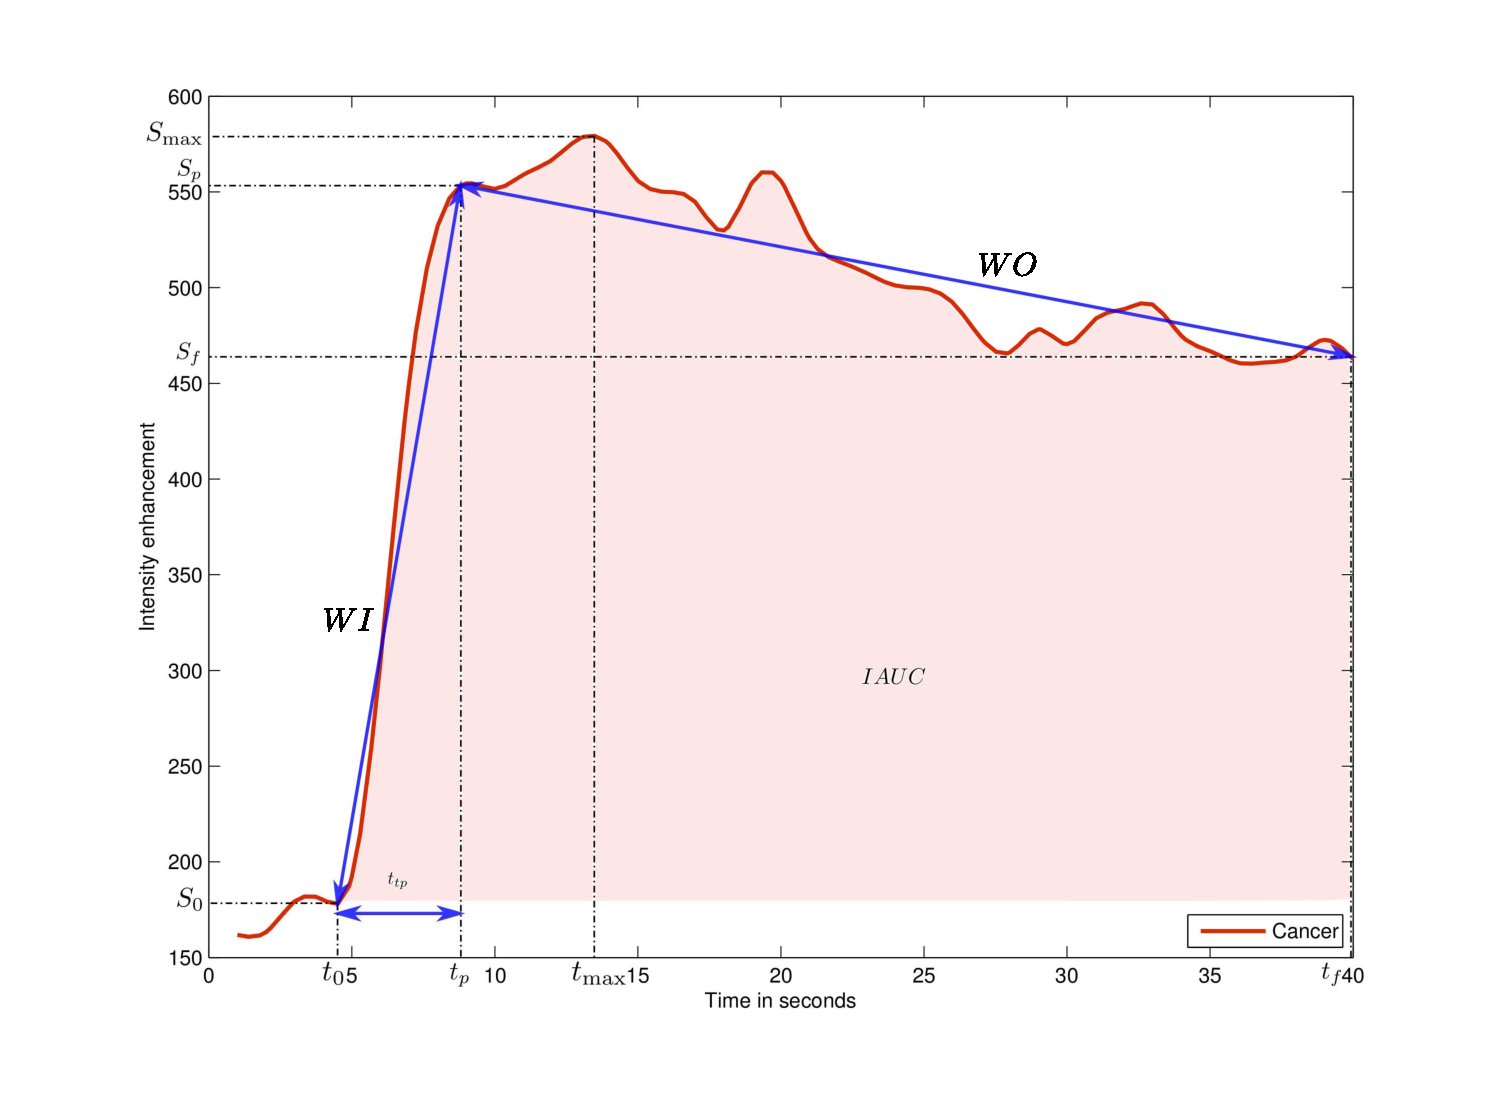
\includegraphics[width=\linewidth]{04_data_classification/06_feature_detection/figures/dce/dce_cancer_parameters.eps}
	\caption{Graphical representation of the different semi-quantitative features used for \ac{dce}-\ac{mri} analysis.}
	\label{fig:dceparam}
\end{figure}

\item[$-$] \textbf{\textit{Semi-quantitative approach:}} Semi-quantitative approaches are based on modelling mathematically the \ac{dce} time series. The parameters modelling the signal are commonly used mainly due to the simplicity to compute them. Parameters included in semi-quantitative analysis are summarized in Tab. \ref{tab:semiqua} and also graphically depicted in Fig. \ref{fig:dceparam}. A set of time features corresponding to specific amplitude level (start, maximum and end) are extracted. Then, derivative and integral are also considered as discriminative and are commonly computed.

\item[$-$] \textbf{\textit{Quantitative approach:}} As presented in Sect. \ref{subsubsec:mrimrsi}, quantitative approaches correspond to mathematical-pharmacokinetic models based on physiological exchanges. Four different models have been used in \ac{cad} systems. 

The most common model reviewed was the Brix model (\cite{Artan2009,Artan2010,Sung2011,Liu2009,Ozer2009,Ozer2010}). This model is formalized such as:
\begin{equation}
	\frac{S(t)}{S(0)} = 1 + A k_{ep} \left( \frac{\exp( -k_{ep} t ) - \exp( -k_{el} t )}{k_{el} - k_{ep}} \right) \ ,
	\label{eq:brixmod}
\end{equation}

\noindent where $S(\cdot)$ is the \ac{dce} signal, $A$ is the parameter simulating the tissue properties, $k_{el}$ is the parameter related to the first-order elimination from the plasma compartment, $k_{ep}$ is the parameter of the transvascular permeability.

Thus, the parameters $k_{ep}$, $k_{el}$ and $A$ are computed and used as features.

Tofts model (\cite{Tofts1997}) was used by \cite{Langer2009,Giannini2013,Niaf2011,Niaf2012,Mazzetti2011}. The \ac{dce} signal relative to the concentration is then modelled such as:
\begin{equation}
	C_t(t) = v_p C_p(t) + K_{trans} \int_{0}^{t} C_p(\tau) \exp( -k_{ep}(t-\tau) ) \ d\tau \ ,
	\label{eq:tofts} 
\end{equation}

\noindent where $C_t(\cdot)$ is the concentration of the medium, $C_p(\cdot)$ is the \ac{aif} which have to be estimated apart, $K_{trans}$ is the parameter related to the diffuse transport of media across the capillary endothelium, $k_{ep}$ is the parameter related to the exchanges back into the vascular space and $v_e$ is the extravascular-extracellular space fraction such as $v_e = 1 - v_p$. 

Thus, the parameters $K_{trans}$, $k_{ep}$ and $v_e$ are computed and used as features.

\cite{Mazzetti2011} and \cite{Giannini2013} employed two others empirical models. A Weibull function was used and can be formalized such as:
\begin{equation}
	S(t) = A t \exp( -t^{B} ) \ ,
	\label{eq:weibull}
\end{equation}

\noindent where $A$ and $B$ are the two parameters which have to be inferred.

The other empirical model is called phenomenological universalities model (\cite{Castorina2006}) which can be formalized:
\begin{equation}
	S(t) = \exp \left( r t + \frac{1}{\beta} a_0 - r ( \exp( \beta t ) - 1 ) \right) \ ,
	\label{eq:pun}
\end{equation}

\noindent where the parameters $\beta$, $a_0$ and $r$ are inferred by using curve fitting approach.

\end{enumerate}

\subsubsection{\ac{mrsi}-based features}

\setenumerate{listparindent=\parindent,itemsep=10px}
\setlist{noitemsep}
\begin{enumerate}[leftmargin=*]

\item[$-$] \textbf{\textit{Whole spectra approach:}} As for the \ac{dce} analysis, one common approach is to incorporate the whole \ac{mrsi} spectra in the feature vector to classify (\cite{Kelm2007,Parfait2012,Tiwari2007,Tiwari2009,Tiwari2013,Tiwari2009a,Tiwari2010,Viswanath2008a,Matulewicz2013}) Sometimes post-processing involving dimension reduction methods is perform to reduce the complexity during the classification as it will be presented in Sect. \ref{subsec:featureselectionextraction}.

\item[$-$] \textbf{\textit{Quantification approach:}} We cab recall that in \ac{mrsi} only few biological markers (cf., choline, creatine and citrate metabolites mainly) are known to be useful to discriminate \ac{cap} and healthy tissue. Then, quantification of these metabolite concentrations are considered as feature for further classification. In order to perform this quantification, four different approaches have been used. QUEST (\cite{Ratiney2005}), AMARES (\cite{Vanhamme1997}) and VARPRO (\cite{Coleman1993}) were used by \cite{Kelm2007} which are all time-domain quantification methods varying by the type of pre-knowledge embedded and the optimization approaches used to solve the quantification problem. Unlike the previous method, \cite{Parfait2012} used the LcModel approach (\cite{Provencher1993}) which solves the optimization problem in the frequency domain.

Once the different concentrations are computed, \cite{Kelm2007} calculated the relative concentrations (Eq. \eqref{eq:ratio1} and \eqref{eq:ratio2}) and used them as features. However, \cite{Parfait2012} used each metabolite concentrations individually.

\begin{eqnarray}
	R_1 & = & \frac{ [ \text{Cho} ] + [ \text{Cr} ]}{[ \text{Cit} ]} \ . \label{eq:ratio1} \\
	R_2 & = & \frac{[ \text{Cit} ]}{[\text{Cho}]+[\text{Cr}]+[\text{Cit}]} \ , \label{eq:ratio2}
\end{eqnarray}

\noindent where $\text{Cit}$, $\text{Cho}$ and $\text{Cr}$ are the concentration of citrate, choline and creatine respectively.

\item[$-$] \textbf{\textit{Wavelet decomposition approach:}} \cite{Tiwari2012} performed a wavelet packet decomposition (\cite{Coifman1992}) by using the Haar wavelet basis function and use the coefficients of this decomposition as features for further classification.

\end{enumerate}